Das Verfahren zur Bestimmung der deflektometrischen Registrierung konnte bestimmte Fehlstellen auch bei der Durchlichtauswertung sichtbar machen.
Allerdings sind schwächere Kratzer und Gravuren untergegangen.
Aus dem Grund wird zum Vergleich das Brillenglas 1 genommen und durch den Aufbau für die Spiegelbildauswertung (siehe rechtes Teilbild aus Abbildung \ref{tikz:abbAufbauFotos}) geprüft.
Wie auch im Abschnitt \ref{sub:spiegelbildAuswertungLichtstreuung} kann für Brillenglas 1 der Rückseitenreflex durch die Polarisation und Färbung nahezu vollständig vermieden werden.
Die Spiegelbildauswertung ermöglicht auch die Anwendung des Verfahrens für nicht-transparente spiegelnde Objekte, weshalb die Keramikobjekte 1 und 2 aus Abbildung \ref{tikz:abbStreifenaufnahmenSpLichtstreuung} zur Prüfung herangezogen werden.

\p
Unter der Spiegelung eines sinusoidalen Streifenmusters nach den Parametern aus Tabelle \ref{tab:paramDeflektometrischRegistrierung} werden die Prüfobjekte in Abbildung \ref{tikz:abbSinusStreifenmusterSpiegel} dargestellt.

% Abbildung: Aufnahmen mit sinusoidalen Streifenmustern
{
	\begin{figure}[H]
		\centering
		\begin{adjustbox}{width=\textwidth}
	\begin{tikzpicture}[every node/.style={inner sep=0,outer sep=0}]
		% Bilder
		\node [anchor=north west] (img1) at (0,0) {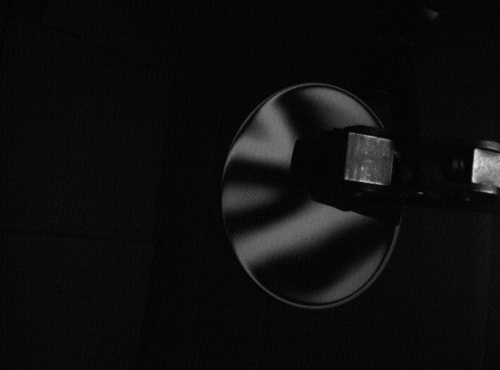
\includegraphics[width=.31\textwidth]{05_ergebnisse/ergDeflektometrischeRegistrierung/spiegelbildAuswertungDeflektometrischeRegistrierung/figures/brillenglas_1_streifenmuster}};
		
		\node [anchor=north west] (img2) at (0.345\textwidth,0) {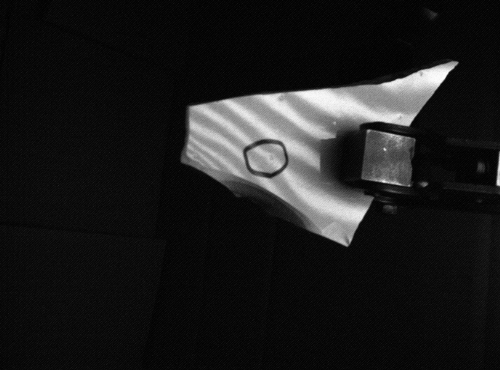
\includegraphics[width=.31\textwidth]{05_ergebnisse/ergDeflektometrischeRegistrierung/spiegelbildAuswertungDeflektometrischeRegistrierung/figures/keramikobjekt_1_streifenmuster}};
		
		\node [anchor=north west] (img3) at (0.69\textwidth,0) {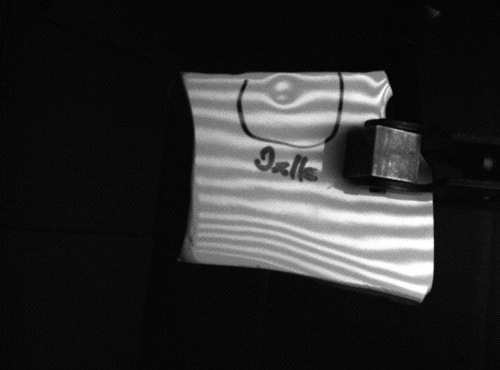
\includegraphics[width=.31\textwidth]{05_ergebnisse/ergDeflektometrischeRegistrierung/spiegelbildAuswertungDeflektometrischeRegistrierung/figures/keramikobjekt_2_streifenmuster}};
		
		% Captions
		\node [below=0.2cm of img1] (cap1) {Brillenglas 1};
		\node [below=0.2cm of img2] (cap2) {Keramikobjekt 1};
		\node [below=0.2cm of img3] (cap3) {Keramikobjekt 2};
	\end{tikzpicture}
\end{adjustbox}
\caption[Aufnahmen der Prüfobjekte unter Spiegelung der sinusoidalen Streifenmuster]{Aufnahmen der Prüfobjekte unter Spiegelung der sinusoidalen Streifenmuster}
		\label{tikz:abbSinusStreifenmusterSpiegel}
	\end{figure}
}

\noindent
Nach der Bestimmung der deflektometrischen Registrierung der Prüfobjekte können daraus Bilder erstellt werden (siehe Definition \ref{def:graphDeflektometrischeRegistrierung}):

% Abbildung: Bilder der deflektometrische Registrierung der Zeilen
{
	\begin{figure}[H]
		\centering
		\begin{adjustbox}{width=\textwidth}
	\begin{tikzpicture}[every node/.style={inner sep=0,outer sep=0}]
		% Bilder
		\node [anchor=north west] (img1) at (0,0) {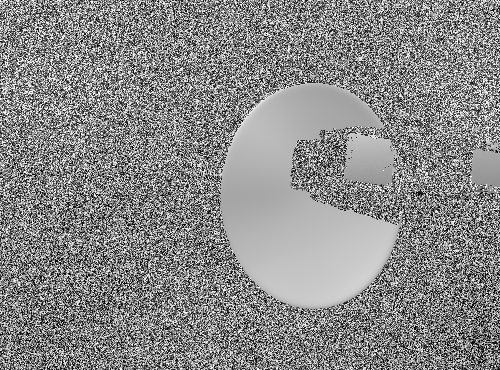
\includegraphics[width=.31\textwidth]{05_ergebnisse/ergDeflektometrischeRegistrierung/spiegelbildAuswertungDeflektometrischeRegistrierung/figures/brillenglas_1_registrierung}};
		
		\node [anchor=north west] (img2) at (0.345\textwidth,0) {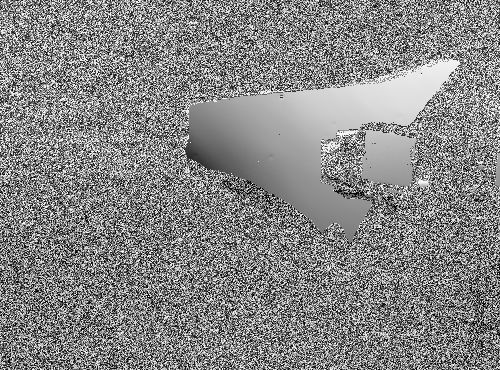
\includegraphics[width=.31\textwidth]{05_ergebnisse/ergDeflektometrischeRegistrierung/spiegelbildAuswertungDeflektometrischeRegistrierung/figures/keramikobjekt_1_registrierung}};
		
		\node [anchor=north west] (img3) at (0.69\textwidth,0) {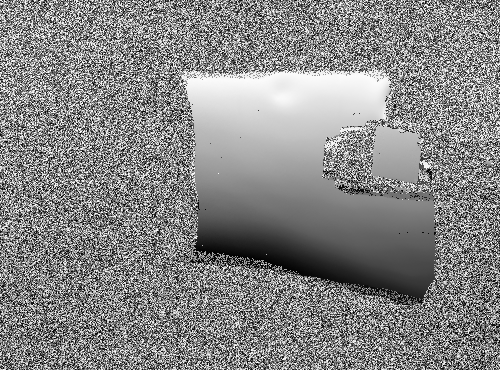
\includegraphics[width=.31\textwidth]{05_ergebnisse/ergDeflektometrischeRegistrierung/spiegelbildAuswertungDeflektometrischeRegistrierung/figures/keramikobjekt_2_registrierung}};
		
		% Captions
		\node [below=0.2cm of img1] (cap1) {Brillenglas 1};
		\node [below=0.2cm of img2] (cap2) {Keramikobjekt 1};
		\node [below=0.2cm of img3] (cap3) {Keramikobjekt 2};
	\end{tikzpicture}
\end{adjustbox}
\caption[Bilder der deflektometrischen Registrierung der Zeilen bei der Spiegelbildauswertung]{Bilder der deflektometrischen Registrierung der Zeilen bei der Spiegelbildauswertung.}
		\label{tikz:abbDeflectometricRegistrationsSpiegel}
	\end{figure}
}

\noindent
In den Bildern der deflektometrischen Zeilenregistrierung tauchen in den zu untersuchenden Objekten einzelne Bildpunkte auf, deren Grauwerte nicht zu der Umgebung passen.
Diese Ausreißer haben für die Oberflächenform keine größere Bedeutung und entstehen z. B. durch Messfehler, Fremdlicht oder die angestrahlte Abschirmung, die von innen Licht auf das Prüfobjekt reflektiert.
Durch Anwendung des Medianfilters zur Glättung des Bildes, kann man diese Störung entfernen.
Anschließend kann auch für diese Objekte zur Auswertung der deflektometrischen Registrierung die Ableitung der geglätteten Bilder in Richtung der Zeilen gebildet werden:

% Abbildung: Bilder der Ableitung der deflektometrische Registrierung der Zeilen
{
	\begin{figure}[H]
		\centering
		\begin{adjustbox}{width=\textwidth}
	\begin{tikzpicture}[every node/.style={inner sep=0,outer sep=0}]
		% Bilder
		\node [anchor=north west] (img1) at (0,0) {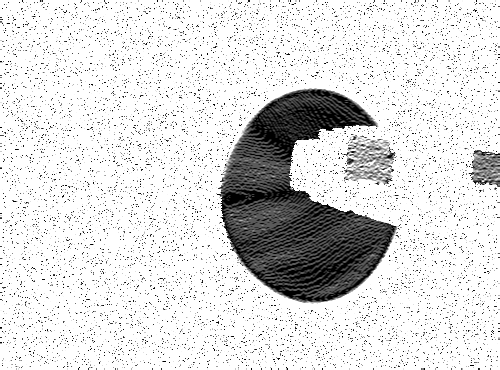
\includegraphics[width=.31\textwidth]{05_ergebnisse/ergDeflektometrischeRegistrierung/spiegelbildAuswertungDeflektometrischeRegistrierung/figures/brillenglas_1_ableitung}};
		
		\node [anchor=north west] (img2) at (0.345\textwidth,0) {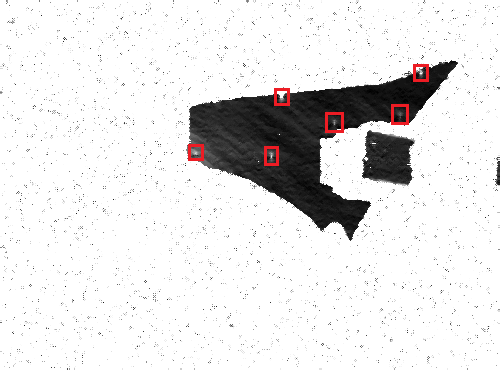
\includegraphics[width=.31\textwidth]{05_ergebnisse/ergDeflektometrischeRegistrierung/spiegelbildAuswertungDeflektometrischeRegistrierung/figures/keramikobjekt_1_ableitung}};
		
		\node [anchor=north west] (img3) at (0.69\textwidth,0) {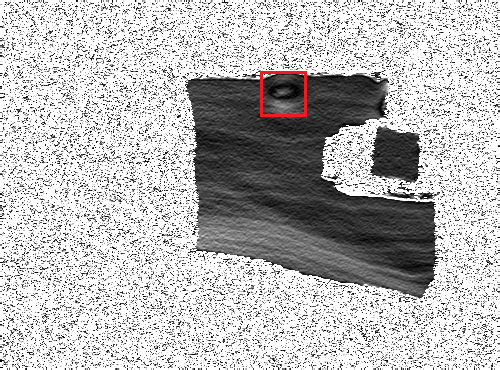
\includegraphics[width=.31\textwidth]{05_ergebnisse/ergDeflektometrischeRegistrierung/spiegelbildAuswertungDeflektometrischeRegistrierung/figures/keramikobjekt_2_ableitung}};
		
		% Captions
		\node [below=0.2cm of img1] (cap1) {Brillenglas 1};
		\node [below=0.2cm of img2] (cap2) {Keramikobjekt 1};
		\node [below=0.2cm of img3] (cap3) {Keramikobjekt 2};
	\end{tikzpicture}
\end{adjustbox}
\caption[Ableitungen der Bilder der deflektometrischen Registrierung der Zeilen bei der Spiegelbildauswertung]{Ableitung der Bilder der deflektometrischen Registrierung der Zeilen bei der Spiegelbildauswertung.}
		\label{tikz:abbAbleitungRegistrierungSpiegel}
	\end{figure}
}

\noindent
Genau wie bei der Durchlichtauswertung dieses Verfahren lassen sich bei dem Brillenglas 1 in Abbildung \ref{tikz:abbAbleitungRegistrierungSpiegel} keine größeren Auffälligkeiten feststellen.
Es lassen sich demnach nicht wie im Abschnitt \ref{sub:spiegelbildAuswertungLichtstreuung} Fehlstellen oder die Gravur der Brillenkennzeichnung erkennen.
Auf den Keramikobjekten 1 und 2 erkennt man allerdings abgesehen von den Krümmungsverläufen der Oberfläche weitere Abweichungen.
In Abbildung \ref{tikz:abbAbleitungRegistrierungSpiegel} sind die Auffälligkeiten durch rote Rechtecke markiert.
Beim Keramikobjekt 1 handelt es sich hierbei um sogenannte  \glqq Pickel\grqq ~auf der Oberfläche.
Auf der Oberfläche des Keramikobjekts 2 befindet sich im roten Rechteck eine Delle bzw. Wölbung in die Oberfläche.

\p
Als Alternative zur Auswertung der deflektometrischen Registrierung über die Ableitung, wird eine Auswertung über die Krümmungsberechnung durch den sogenannten Mexican Hat-Operator durchgeführt: 

% Abbildung: Bilder des Mexican Hat Filter angewandt auf die deflektometrische Registrierung der Zeilen
{
	\begin{figure}[H]
		\centering
		\begin{adjustbox}{width=\textwidth}
	\begin{tikzpicture}[every node/.style={inner sep=0,outer sep=0}]
		% Bilder
		\node [anchor=north west] (img1) at (0,0) {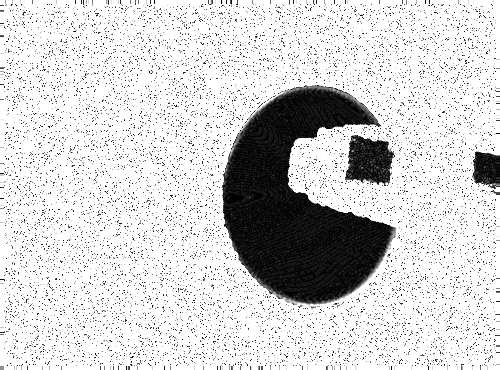
\includegraphics[width=.31\textwidth]{05_ergebnisse/ergDeflektometrischeRegistrierung/spiegelbildAuswertungDeflektometrischeRegistrierung/figures/brillenglas_1_mexican}};
		
		\node [anchor=north west] (img2) at (0.345\textwidth,0) {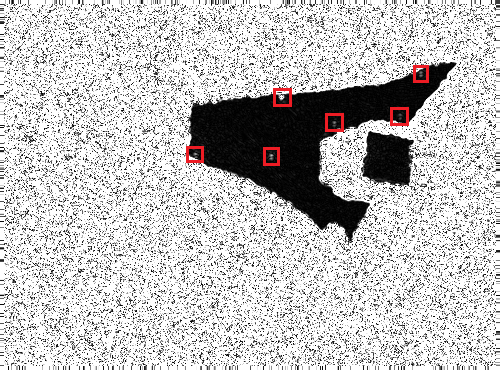
\includegraphics[width=.31\textwidth]{05_ergebnisse/ergDeflektometrischeRegistrierung/spiegelbildAuswertungDeflektometrischeRegistrierung/figures/keramikobjekt_1_mexican}};
		
		\node [anchor=north west] (img3) at (0.69\textwidth,0) {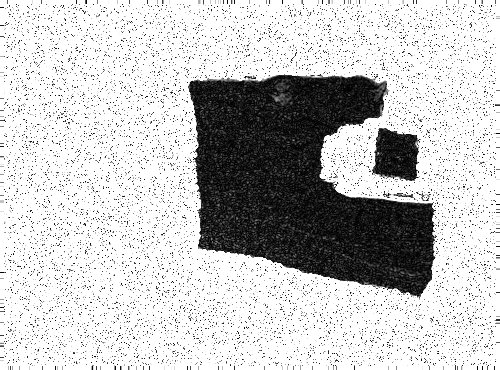
\includegraphics[width=.31\textwidth]{05_ergebnisse/ergDeflektometrischeRegistrierung/spiegelbildAuswertungDeflektometrischeRegistrierung/figures/keramikobjekt_2_mexican}};
		
		% Captions
		\node [below=0.2cm of img1] (cap1) {Brillenglas 1};
		\node [below=0.2cm of img2] (cap2) {Keramikobjekt 1};
		\node [below=0.2cm of img3] (cap3) {Keramikobjekt 2};
	\end{tikzpicture}
\end{adjustbox}
\caption[Mexican Hat-Filter angewandt auf die Bilder der deflektometrischen Registrierung der Zeilen]{Mexican Hat-Filter angewandt auf die Bilder der deflektometrischen Registrierung der Zeilen.}
		\label{tikz:abbMexicanHatRegistrierung}
	\end{figure}
}

\noindent
Auch in Abbildung \ref{tikz:abbMexicanHatRegistrierung} erkennt man im Brillenglas keine Abweichungen der Oberflächen\-krümmung.
Auf den Keramikobjekten 1 und 2 erkennt man an den in Abbildung \ref{tikz:abbAbleitungRegistrierungSpiegel} markierten Fehlstellen auch Auffälligkeiten in Abbildung \ref{tikz:abbMexicanHatRegistrierung}.

%TODO Abschluss der Section?